% Informe resumido: visión (YOLO + estéreo) de Arturito R2D2 — Grupo 2, FIUNA Mecatrónica, 2026S2
% Compilar desde esta carpeta:  pdflatex informe_vision && pdflatex informe_vision
\documentclass[11pt,a4paper]{article}

\usepackage[T1]{fontenc}
\usepackage[utf8]{inputenc}
\usepackage[spanish,es-noshorthands,es-tabla]{babel}
\usepackage{lmodern}
\usepackage{microtype}
\usepackage[a4paper,margin=2.3cm]{geometry}
\usepackage{amsmath}
\usepackage{icomma}
\usepackage[table]{xcolor}
\usepackage{graphicx}
\usepackage{float}
\usepackage{caption}
\usepackage{subcaption}
\usepackage{booktabs}
\usepackage{enumitem}
\usepackage{tikz}
\usetikzlibrary{positioning,arrows.meta}
\usepackage[hidelinks]{hyperref}

\definecolor{acento}{HTML}{1F6F8B}
\definecolor{naranja}{HTML}{D98E04}
\setlist{itemsep=2pt,topsep=4pt}
\newcommand{\cod}[1]{\texttt{#1}}

\tikzset{
  caja/.style={draw=acento,thick,rounded corners=3pt,fill=acento!8,align=center,minimum height=1cm,inner sep=5pt},
  nodo/.style={draw=naranja,thick,rounded corners=3pt,fill=naranja!10,align=center,minimum height=1cm,inner sep=5pt},
  datos/.style={-{Stealth[length=6pt]},thick}
}

\title{\textbf{Visión del robot recolector de limones}\\[4pt]
\large Detección con YOLO y localización con visión estéreo: qué está hecho}
\author{Grupo 2 --- Arturito R2D2\\FIUNA, Ingeniería Mecatrónica, Robótica II (2026S2)}
\date{20 de octubre de 2026}

\begin{document}
\maketitle

\section*{Resumen}
El robot tiene que encontrar un limón y saber dónde está en 3D para que el brazo lo agarre. Para eso usa dos
cámaras en una Raspberry Pi 5: una red \textbf{YOLO} dice \emph{qué} es un limón en la imagen y la
\textbf{visión estéreo} dice \emph{a qué distancia} está. Toda la cadena corre en la Pi con ROS~2 Jazzy y publica la
posición del limón en el tópico \cod{/limon/posicion}.

En el laboratorio, con un limón real, \textbf{el detector lo encuentra con confianza mediana de 0,80 y la posición
tiene un error 3D máximo de 17~mm} (la guía pide 35~mm o menos). Falta la prueba en campo y separar el limón en
cosechable, no cosechable u obstáculo.

\section{Hardware}
\begin{itemize}
  \item \textbf{Cámaras:} dos Raspberry Pi Camera Module 3 NoIR (sensor IMX708) por CSI, montadas en un soporte
        rígido a 90~mm una de otra (\emph{baseline}). Imagen de 640 × 480 con el sensor completo y foco fijo.
  \item \textbf{Computadora:} Raspberry Pi 5 con Ubuntu 24.04 y ROS~2 Jazzy. No usa GPU: todo corre en la CPU.
  \item El software está en un repositorio propio (\cod{vision\_estereo}) y el entrenamiento del detector en un
        cuaderno de Google Colab.
\end{itemize}

\section{Cómo funciona la cadena}

\begin{figure}[H]
\centering
\resizebox{\textwidth}{!}{%
\begin{tikzpicture}[every node/.append style={font=\small}]
  \node[caja] (cl) at (0,0) {cámara\\izquierda};
  \node[caja] (cr) at (0,-2.2) {cámara\\derecha};
  \node[nodo] (rl) at (3.2,0) {rectificar};
  \node[nodo] (rr) at (3.2,-2.2) {rectificar};
  \node[nodo] (sg) at (6.8,-1.1) {disparidad\\(SGBM)};
  \node[nodo] (yo) at (6.8,1.4) {YOLO\\(qué es)};
  \node[nodo] (lo) at (10.2,-1.1) {localizador\\(dónde está)};
  \node[caja] (out) at (13.6,-1.1) {posición 3D\\\cod{/limon/posicion}};
  \draw[datos] (cl) -- (rl); \draw[datos] (cr) -- (rr);
  \draw[datos] (rl) -- (sg); \draw[datos] (rr) -- (sg);
  \draw[datos] (rl) |- (yo);
  \draw[datos] (sg) -- (lo);
  \draw[datos] (yo) -| (lo);
  \draw[datos] (lo) -- (out);
\end{tikzpicture}}
\caption{De las dos imágenes a la posición del limón.}
\end{figure}

\begin{enumerate}
  \item Las dos cámaras toman una imagen cada una.
  \item Se \textbf{rectifican}: se corrigen para que un mismo punto quede en la misma fila de las dos imágenes.
  \item \textbf{YOLO} busca limones en la imagen izquierda y devuelve una caja alrededor de cada uno.
  \item El algoritmo \textbf{SGBM} compara las dos imágenes y calcula la disparidad (cuánto se corre cada punto
        entre una cámara y la otra). Cuanto más cerca está el objeto, más se corre.
  \item El \textbf{localizador} toma los puntos dentro de la caja del limón, separa el limón de las hojas que están
        detrás y calcula su posición $X$, $Y$, $Z$ en metros.
\end{enumerate}

\section{Detección con YOLO}

\begin{itemize}
  \item \textbf{Modelo:} YOLO26n (la versión más chica), con una sola clase: \cod{limon}.
  \item \textbf{Entrenamiento:} en Google Colab (GPU T4), con imágenes de datasets públicos de Roboflow.
  \item \textbf{En la Pi:} exportado a \textbf{NCNN}, un formato optimizado para procesadores ARM. Corre a 23
        imágenes por segundo solo y a 7--9 dentro de la cadena completa.
\end{itemize}

\begin{table}[H]
\centering
\begin{tabular}{@{}lc@{}}
\toprule
\textbf{Métrica (conjunto de prueba)} & \textbf{Valor} \\
\midrule
Precisión (de lo que marca, cuánto es limón) & 0,953 \\
Recobrado (de los limones, cuántos encuentra) & 0,977 \\
mAP50 & 0,978 \\
mAP50-95 & 0,814 \\
\bottomrule
\end{tabular}
\caption{Resultados del detector sobre 285 imágenes de prueba (173 limones, 200 imágenes sin limón).}
\end{table}

Estos números son optimistas, porque las imágenes de prueba vienen de las mismas fuentes que las de entrenamiento.
Por eso se probó también con un \textbf{limón real} frente a las cámaras del robot: lo detectó con confianza
mediana de \textbf{0,80}.

\section{Visión estéreo}

\subsection{La idea}
Es como mirar con los dos ojos: un objeto cercano se ``corre'' más entre una cámara y otra que uno lejano. Si $d$ es
ese corrimiento en píxeles (\emph{disparidad}), la distancia es
\[
  Z = \frac{f \cdot B}{d}
\]
donde $f$ es la distancia focal (654~px) y $B$ la separación entre cámaras (89,5~mm). Por ejemplo, un limón a
40~cm se corre 146~px y uno a 90~cm, 65~px. El error crece con el cuadrado de la distancia, por eso conviene mirar
el limón de cerca.

\subsection{Calibración}
Para usar la fórmula hay que conocer bien las cámaras. Se fotografió un tablero de ajedrez (9 × 6 esquinas, cuadros de
25~mm) en 34 posiciones distintas y OpenCV calculó la focal, la distorsión de cada lente y la posición de una cámara
respecto de la otra.

\begin{figure}[H]
\centering
\begin{subfigure}{0.45\textwidth}\centering
  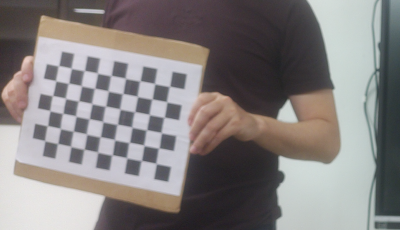
\includegraphics[width=\linewidth]{figuras/calib_left.png}\caption{Cámara izquierda}
\end{subfigure}\hfill
\begin{subfigure}{0.45\textwidth}\centering
  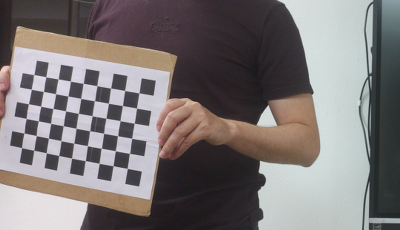
\includegraphics[width=\linewidth]{figuras/calib_right.png}\caption{Cámara derecha}
\end{subfigure}
\caption{Uno de los 34 pares de imágenes de la calibración (recortados). El tablero aparece corrido entre las dos
cámaras: esa es la disparidad.}
\end{figure}

\begin{table}[H]
\centering
\begin{tabular}{@{}ll@{}}
\toprule
\textbf{Resultado de la calibración} & \textbf{Valor} \\
\midrule
Error de reproyección (RMS) & 0,36~px \\
Error vertical entre imágenes rectificadas & 0,08~px (medio) \\
Separación entre cámaras calculada & 89,5~mm (con regla: 90~mm) \\
Distancia focal & 654,3~px \\
Rango de trabajo & 0,38 a 0,96~m \\
\bottomrule
\end{tabular}
\caption{Calibración en uso (soporte rígido, 1 de octubre). Un error menor a 0,5~px se considera bueno.}
\end{table}

\subsection{Disparidad y localización}
Se probaron dos algoritmos de OpenCV: \textbf{BM} (rápido, unas 10 imágenes por segundo, pero ruidoso) y
\textbf{SGBM} (más lento, unas 2,5 por segundo, pero mucho más limpio). Se eligió \textbf{SGBM}, porque para
agarrar el limón importa más la precisión que la velocidad: el robot se detiene y recién entonces localiza.

Dentro de la caja de YOLO hay limón y también hojas o ramas detrás. El localizador ordena las profundidades de los
puntos, corta donde hay un salto de más de 5~cm y se queda con el grupo más cercano: ese es el limón.

\section{Resultados con un limón real}

Se colocó un limón a distancias conocidas, medidas con cinta métrica, y se comparó con lo que daba el sistema.

\begin{table}[H]
\centering
\begin{tabular}{@{}lcccc@{}}
\toprule
\textbf{Distancia real [mm]} & 400 & 550 & 700 & 900 \\
\midrule
Medida por el estéreo (SGBM) [mm] & 409 & 554 & 713 & 915 \\
Error [mm] & +9 & +4 & +13 & +15 \\
\bottomrule
\end{tabular}
\caption{Limón en el eje de la cámara.}
\end{table}

\begin{table}[H]
\centering
\begin{tabular}{@{}cccccc@{}}
\toprule
\textbf{Real Z} & \textbf{Real X} & \textbf{Medido Z} & \textbf{Medido X} & \textbf{Error Z} & \textbf{Error X} \\
\midrule
400 & $-$100 & 412 & $-$97 & +12 & +3 \\
400 & +70 & 404 & +87 & +4 & +17 \\
550 & $-$150 & 558 & $-$160 & +8 & $-$10 \\
550 & +100 & 552 & +97 & +2 & $-$3 \\
700 & $-$200 & 705 & $-$201 & +5 & $-$1 \\
700 & +120 & 713 & +116 & +13 & $-$4 \\
\bottomrule
\end{tabular}
\caption{Limón corrido a los costados (todo en mm; $X$ medido con regla).}
\end{table}

\begin{itemize}
  \item \textbf{Error 3D máximo: 17~mm.} La guía (requisito B5) pide 35~mm o menos: \textbf{se cumple en el
        laboratorio}.
  \item El ruido entre mediciones seguidas es menor a 2~mm.
  \item Queda un desfase de alrededor de +1~cm en la distancia, en parte porque la cinta se midió desde el frente de
        la lente y no desde el centro óptico.
\end{itemize}

\section{Limitaciones conocidas}
\begin{itemize}
  \item \textbf{Zona ciega:} un limón en el cuarto izquierdo de la imagen izquierda se detecta pero no se puede
        localizar (no aparece en la cámara derecha dentro del rango buscado).
  \item \textbf{Cámaras no sincronizadas:} cada una dispara por su cuenta, así que se localiza con el robot quieto.
  \item \textbf{Cámaras NoIR} (sin filtro infrarrojo): al sol los colores salen rosados y el detector podría fallar.
  \item \textbf{Una sola clase:} todavía no distingue entre limón cosechable, no cosechable u obstáculo.
\end{itemize}

\section{Qué falta}
\begin{enumerate}
  \item \textbf{Prueba de campo:} un limón en una planta, a 40--90~cm, al aire libre (la herramienta de medición ya
        está preparada).
  \item Probar las cámaras NoIR al sol.
  \item Reentrenar el detector con tres clases: cosechable, no cosechable y obstáculo u oclusión (requisito B3).
  \item Medir la posición de las cámaras respecto del brazo, con el soporte montado en el robot, para pasar la
        posición del limón al sistema de coordenadas del brazo.
\end{enumerate}

\end{document}
